\documentclass[shownotes,11pt, aspectratio=169]{beamer}

\usepackage{pgfpages}
% These slides also contain speaker notes. You can print just the slides,
% just the notes, or both, depending on the setting below. Comment out the want
% you want.
\setbeameroption{hide notes} % Only slide
%\setbeameroption{show only notes} % Only notes
%\setbeameroption{show notes on second screen=right} % Both

\usepackage{helvet}
\usepackage[default]{Fira Sans}
\usepackage{array}
\usepackage{caption}
%\usepackage[clean]{svg}
\usepackage{tikz}
\usepackage{verbatim}
\setbeamertemplate{note page}{\pagecolor{yellow!5}\insertnote}
\usetikzlibrary{positioning}
\usetikzlibrary{snakes}
\usetikzlibrary{calc}
\usetikzlibrary{arrows}
\usetikzlibrary{decorations.markings}
\usetikzlibrary{shapes.misc}
\usetikzlibrary{matrix,shapes,arrows,fit,tikzmark}
\usepackage{amsmath}
\usepackage{mathpazo}
\usepackage{hyperref}
\usepackage{lipsum}
\usepackage{multimedia}
\usepackage{graphicx}
\usepackage{multirow}
\usepackage{graphicx}
\usepackage{dcolumn}
\usepackage{tfrupee}
\usepackage{bbm}
\newcolumntype{d}[0]{D{.}{.}{5}}

\usepackage{changepage}
\usepackage{appendixnumberbeamer}
\newcommand{\beginbackup}{
   \newcounter{framenumbervorappendix}
   \setcounter{framenumbervorappendix}{\value{framenumber}}
   \setbeamertemplate{footline}
   {
     \leavevmode%
     \hline
     box{%
       \begin{beamercolorbox}[wd=\paperwidth,ht=2.25ex,dp=1ex,right]{footlinecolor}%
%         \insertframenumber  \hspace*{2ex} 
       \end{beamercolorbox}}%
     \vskip0pt%
   }
 }
\newcommand{\backupend}{
   \addtocounter{framenumbervorappendix}{-\value{framenumber}}
   \addtocounter{framenumber}{\value{framenumbervorappendix}} 
}


\usepackage{graphicx}
\usepackage[space]{grffile}
\usepackage{booktabs}

% These are my colors -- there are many like them, but these ones are mine.
\definecolor{blue}{RGB}{0,114,178}
\definecolor{red}{RGB}{213,94,0}
\definecolor{yellow}{RGB}{240,228,66}
\definecolor{green}{RGB}{0,158,115}

\hypersetup{
  colorlinks=false,
   bookmarks=true,
  linkbordercolor = {white},
  linkcolor = {blue}
}


%% I use a beige off white for my background
\definecolor{MyBackground}{RGB}{255,253,218}

%% Uncomment this if you want to change the background color to something else
\setbeamercolor{background canvas}{bg=MyBackground}

%% Change the bg color to adjust your transition slide background color!
\newenvironment{transitionframe}{
  \setbeamercolor{background canvas}{bg=yellow}
  \begin{frame}}{
    \end{frame}
}

\setbeamercolor{frametitle}{fg=blue}
\setbeamercolor{title}{fg=black}
\setbeamertemplate{footline}[frame number]
\setbeamertemplate{navigation symbols}{} 
\setbeamertemplate{itemize items}{-}
\setbeamercolor{itemize item}{fg=blue}
\setbeamercolor{itemize subitem}{fg=blue}
\setbeamercolor{enumerate item}{fg=blue}
\setbeamercolor{enumerate subitem}{fg=blue}
\setbeamercolor{button}{bg=MyBackground,fg=blue,}



% If you like road maps, rather than having clutter at the top, have a roadmap show up at the end of each section 
% (and after your introduction)
% Uncomment this is if you want the roadmap!
% \AtBeginSection[]
% {
%    \begin{frame}
%        \frametitle{Roadmap of Talk}
%        \tableofcontents[currentsection]
%    \end{frame}
% }
\setbeamercolor{section in toc}{fg=blue}
\setbeamercolor{subsection in toc}{fg=red}
\setbeamersize{text margin left=1em,text margin right=1em} 

\newenvironment{wideitemize}{\itemize\addtolength{\itemsep}{10pt}}{\enditemize}

\title[]{\textcolor{blue}{Macroeconomics: Lecture 2}}
\author[SM]{Sumit Mishra}
\institute[IFMR]{\small{\begin{tabular}{c}
IFMR, Sri City \\
\end{tabular}}}

\date{26 September, 2019}


\begin{document}

%%% TIKZ STUFF
\tikzset{   
        every picture/.style={remember picture,baseline},
        every node/.style={anchor=base,align=center,outer sep=1.5pt},
        every path/.style={thick},
        }
\newcommand\marktopleft[1]{%
    \tikz[overlay,remember picture] 
        \node (marker-#1-a) at (-.3em,.3em) {};%
}
\newcommand\markbottomright[2]{%
    \tikz[overlay,remember picture] 
        \node (marker-#1-b) at (0em,0em) {};%
}
\tikzstyle{every picture}+=[remember picture] 
\tikzstyle{mybox} =[draw=black, very thick, rectangle, inner sep=10pt, inner ysep=20pt]
\tikzstyle{fancytitle} =[draw=black,fill=red, text=white]
%%%% END TIKZ STUFF

% Title Slide
\begin{frame}
\maketitle
%  \centering The views expressed do not necessarily reflect the position of the Federal Reserve Bank of New York or the Federal Reserve System.
\end{frame}

\begin{frame}
\frametitle{Agenda}
\begin{itemize}
 \item Goods Market
         \begin{itemize}
         \item The Demand for Goods
         \item The Determination of Equilibrium Output
         \item Investments \& Savings
         \end{itemize}
\item Financial Market
          \begin{itemize}
           \item Demand for Money
           \item Supply of Money
           \item The Role of Central Bank
           \item Financial Market Equilibrium
           \end{itemize}
\item Material: Blanchard, Chapters 3 \& 4.
\end{itemize}
\end{frame}

%%SLIDE 1
\section{Goods Market}
\begin{frame}{The Composition of GDP}
\begin{wideitemize}
\item \textcolor{red}{Consumption} ($C$) includes spending on fancy phones, \textit{roti}, \textit{kapda}, but not \textit{makaan}. 
\item \textcolor{red}{Investment} ($I$) includes residential plus non-residential investments.
\item \textcolor{red}{Government spending} ($G$) includes purchases made by the government.
\item \textbf{Note:} $G$ does not include \textcolor{red}{government transfers}.
\item \textcolor{red}{Net exports} ($ NX = X - M$)
\end{wideitemize}
\end{frame}

%%%%%
\begin{frame}{The Demand for Goods}
Let demand for goods be $Z$. We can write $Z$ as
\[ Z \equiv C + I + G + NX \]
\\
\vspace{3mm}
\pause
\begin{itemize}
\item Assumption \#1 : All firms produce the same good.
\item Assumption \#2 : Firms are willing to supply any amount of good at given price level $P$.
\item Assumption \#3 : Economy doesn't interact with outside world. ($NX = 0$).
\end{itemize}

\vspace{3mm}
Under these assumptions, the demand is 
\[ Z \equiv C + I + G \]
\end{frame}

%%%%
\begin{frame}{Consumption}
\begin{columns}[T] % align columns
\begin{column}{.52\textwidth}
  \begin{wideitemize}
    \item \textbf{Depends crucially on \textcolor{red}{personal disposable income}.}
    \item Let's just tidy up this messy relationship in form of a neat linear equation.
           \[ C = c_0 + c_1Y_D \]
    \item $c_1$ is the \textcolor{red}{marginal propensity to consume}.
  \end{wideitemize}
\end{column}%
\pause
\hfill%
\begin{column}{.44\textwidth}
  \makebox[\linewidth][c]{
    \resizebox{\linewidth}{!}{
      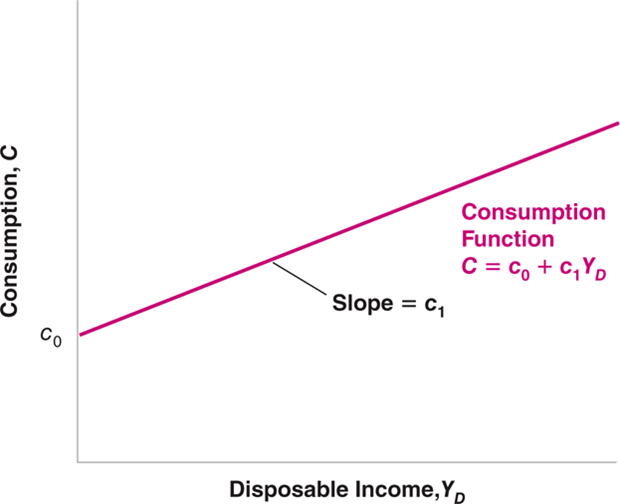
\includegraphics{graphs/L2F1.png}
    }
  }
\end{column}%
\end{columns}
\pause
\[ Y_D \equiv Y - T \]
\[ C = c_0 + c_1(Y - T) \]
\end{frame}

%%%%%%%%%%
\begin{frame}{Investment + Government Spending}
\begin{wideitemize}
\item We assume investments to be fixed. \pause $ I = \bar{I}$.
\pause
\item Just as with investments, we assume that government spending ($G$) and tax levels ($T$) are fixed. 
\end{wideitemize}
\end{frame}

%%%%%%%%
\begin{frame}{The Determination of Equilibrium Output}
The demand for goods is the sum of consumption, investment, and government spending.
\[ Z \equiv C + I + G \]
\pause
\[ Z \equiv c_0 + c_1(Y - T) + \bar{I} + G \]
\pause
How about equilibrium? We assume that \textcolor{red}{firms do not hold inventories}. All that is produced is being sold in the goods market.
\pause
\[ Y = Z \]
\pause
\[ Y = c_0 + c_1(Y - T) + \bar{I} + G \]
\end{frame}

%%%%%
\begin{frame}{The Determination of Equilibrium Output}
Rewrite the last equation:
\[ Y = c_0 + c_1Y - c_1T + \bar{I} + G \]
\pause
Some maths and some sweating later:
\[ Y = \frac{1}{1 - c_1}[c_0 + \bar{I} + G - c_1T] \]
\pause
\begin{wideitemize}
\item[1] The first term on the RHS- $1/(1 - c_1)$ - is called \textcolor{red}{the multiplier}.
\item[2] The second term is known as the \textcolor{green}{autonomous spending}.
\end{wideitemize}
\end{frame}

%%%%%
\begin{frame}{Equilibrium: Graphical Approach}
\begin{columns}[T] % align columns
\begin{column}{.52\textwidth}
  \begin{wideitemize}
    \item[1] Plot $Y$ against $Z$ using the identity between production and income.
    \item[2] Plot $Z$ as a function of income using $Z = (c_0 + \bar{I} + G - c_1T) + c_1Y$.
    \item[3] Equilibrium is at the intersection of the two lines. 
  \end{wideitemize}
\end{column}%
\pause
\hfill%
\begin{column}{.44\textwidth}
  \makebox[\linewidth][c]{
    \resizebox{\linewidth}{!}{
      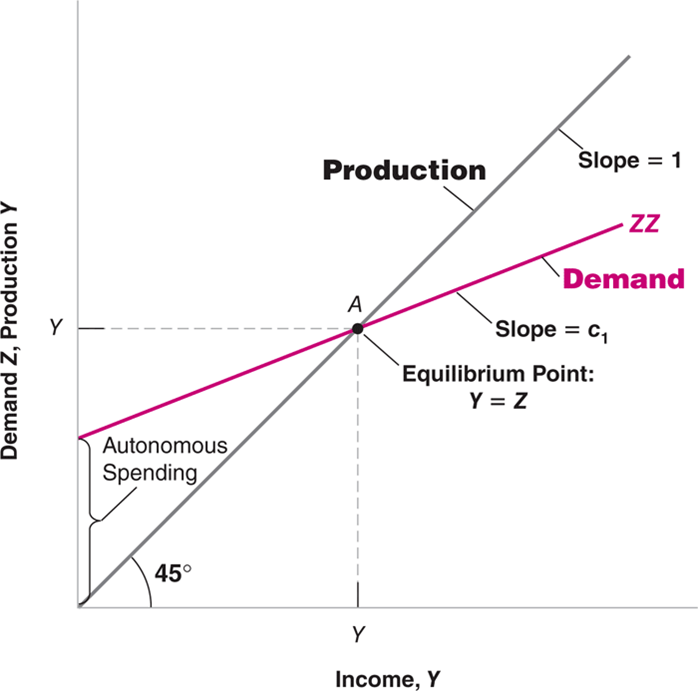
\includegraphics{graphs/L2F2.png}
    }
  }
\end{column}%
\end{columns}
\end{frame}

%%%%
\begin{frame}{Effect of Rising Autonomous Spending on Output}
\begin{columns}[T] % align columns
\begin{column}{.44\textwidth}
  \makebox[\linewidth][c]{
    \resizebox{\linewidth}{!}{
      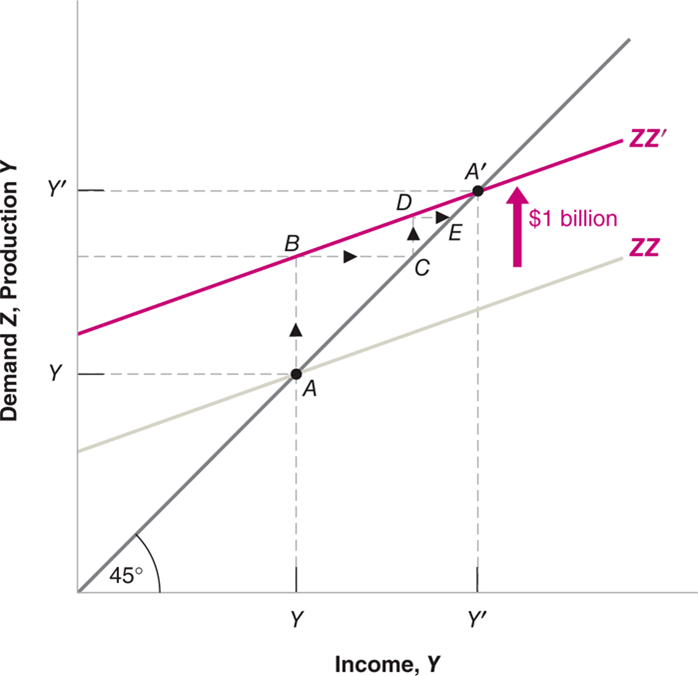
\includegraphics{graphs/L2F3.png}
    }
  }
\end{column}%
\hfill
\begin{column}{.52\textwidth}
  \begin{wideitemize}
    \item[1] The first round increase in demand = AB on the graph.
    \item[2] This increase in demand leads to rise in income = BC on the graph.
    \item[3] The second round increase in demand = CD = $c_1*\Delta Y$
    \item[4] The third round increase in demand = $c_1*c_1*\Delta Y = c_1^2\Delta Y$.
  \end{wideitemize}
\end{column}%
\end{columns}
\end{frame}


%%%%
\begin{frame}{Investment Equals Savings}
Nod to John Maynard Keynes.
\begin{wideitemize}
\item \textbf{Private Savings} ($S$): savings by consumers.
      \[ S^{\text{private}} \equiv Y_D - C \]
\item \textbf{Public Savings}: Net taxes.
      \[ S^{\text{public}} = T - G \]
\pause
\item Let's take a step back and use the demand equation: $Y = C + I + G$
     \[ Y - T - C = I + G - T \]
     \pause
     \[ I = S^{\text{private}} + (T - G) \]    
\item Investment = \textit{private savings} + \textit{public savings}
\end{wideitemize}
Equilibrium in the goods market \textbf{requires} that \textcolor{red}{investment matches savings}. \\
\pause
\textit{What goes around comes around!}
\end{frame}

%%%%
\begin{frame}{Investment-Savings Paradigm: Analytics}
\begin{wideitemize}
\item The decisions to invest/consume are concomitant and identical.
     \[ S = Y - T - C \] \pause
     \[   = Y - T - (c_0 + c_1(Y - T)) \] \pause
     \[ S = -c_0 + (1 - c_1)(Y - T) \]
\item The term $(1 - c_1)$ is known as the \textbf{propensity to save}.
\end{wideitemize}
\end{frame}

\begin{frame}{Investment-Savings Paradigm: Analytics}
\begin{wideitemize}
\item How about investment?
\item Investment = private + public savings.
     \[ I = -c_0 + (1 - c_1)(Y - T) + (T - G) \]
 \pause
 \item If you solve the above equation by assuming $I$ to be a constant, you will get \\
     \[ Y = \frac{1}{1 - c_1}[c_0 + \bar{I} + G - c_1T] \]
\end{wideitemize}
\end{frame}





\begin{frame}
\frametitle{The Meaning of Money}
\begin{quote}
The best things in life are free \\
But you can keep 'em for the birds and bees \\
Now give me money (that's what I want) \\
That's what I want (that's what I want) \\
That's what I want (that's what I want) yeah \\
That's what I want. \\
\end{quote}
The Beatles equate money with wealth. \\
\pause
\vspace*{3mm}

Money is the set of assets in the economy that people regularly use to buy goods and services from
each other. The cash in your wallet is money because you can use it to buy a meal
at a restaurant or a shirt at a clothing store. 
\end{frame}

\section{Introduction}
\begin{frame}{Introduction}
\begin{wideitemize}
\item The difference between ``money'', ``income'', and ``wealth''.
\pause
\item Money works as a \textcolor{red!80}{store of value}, a \textcolor{red!80}{medium of exchange}, and a \textcolor{red!80}{unit of account}.
\end{wideitemize}
\end{frame}

\begin{frame}
\frametitle{Functions of Money}
\textbf{Medium of Exchange} \\
\vspace{3mm}
A medium of exchange is an item that buyers give to sellers when they purchase
goods and services. \\
\vspace{3mm} When you buy a shirt at a clothing store, the store gives
you the shirt, and you give the store your money.  \\
\vspace{3mm}
This transfer of money from buyer to seller allows the transaction to take place. \\
\vspace{3mm}
 When you walk into a store, you are confident that the store will accept your money for the items it is selling
because money is the commonly accepted medium of exchange.
\end{frame}

\begin{frame}
\frametitle{Functions of Money}
\textbf{Unit of Account} \\
\vspace{3mm}
A unit of account is the yardstick people use to post prices and record debts. \\
\vspace{3mm}
When you go shopping, you might observe that a shirt costs Rs.500 and a McD burger
costs Rs.50. \\
\vspace{3mm}
Even though it would be accurate to say that the price of a shirt is 10 McD burgers
and the price of a burger is one-tenth of a shirt, prices are never quoted in
this way.  \\
\vspace{3mm}
Similarly, if you take out a loan from a bank, the size of your future loan
repayments will be measured in dollars, not in a quantity of goods and services.
When we want to measure and record economic value, we use money as the unit
of account.
\end{frame}

\begin{frame}
\frametitle{Functions of Money}
\textbf{A Store of Value} \\
\vspace{3mm}
A store of value is an item that people can use to transfer purchasing power
from the present to the future. \\
\vspace{3mm}
When a seller accepts money today in exchange for a
good or service, that seller can hold the money and become a buyer of another good
or service at another time. \\
\vspace{3mm}
Money is not the only store of value in the economy: A
person can also transfer purchasing power from the present to the future by holding
non-monetary assets such as stocks and bonds. The term wealth is used to refer
to the total of all stores of value, including both money and non-monetary assets
\end{frame}

\section{Demand for Money}
\begin{frame}
Suppose you got a plush corporate job, and over time you are going to accumulate a lot of wealth. But, you are given choice between just two assets: \textit{Money} \& \textit{Bonds}.
\pause
\vspace{5mm}
\begin{wideitemize}
\item Money consists of cash, and \textbf{checkable deposits}. \pause They pay no interest. \pause
\item Bonds pay a positive interest rate, but you can't use them for transactions.
\end{wideitemize}
\pause
\vspace{5mm}
\textcolor{green!90}{The question is: how is your wealth-pie going to be divided between these two?}
\end{frame}

\begin{frame}{Demand for Money}
The proportion will be determined by the following variables: \pause
\vspace{5mm}
\begin{wideitemize}
\item[1] \textcolor{red!90}{Level of transactions}
\item[2] \textcolor{red!90}{The interest rate on bonds}
\end{wideitemize}
\pause
\vspace{5mm}
The money that you save with mutual funds is used to buy government bonds. 
\end{frame}

%%%%%%%
\begin{frame}{Deriving the Demand for Money}
%\begin{frame}{Consumption}
\begin{columns}[T] % align columns
\begin{column}{.52\textwidth}
  \begin{wideitemize}
    \item \textbf{Depends crucially on \textcolor{red}{total number of transactions}.}
    \item Transactions, in turn, depend upon the nominal income.
    \item If income goes up by 10\%, rupee value of transactions also moves in similar direction. 
    \item Let's formalize this relationship.
           \[ M^d =  YL(i) \]
    %\item $c_1$ is the \textcolor{red}{marginal propensity to consume}.
  \end{wideitemize}
\end{column}%
\pause
\hfill%
\begin{column}{.44\textwidth}
  \makebox[\linewidth][c]{
    \resizebox{\linewidth}{!}{
      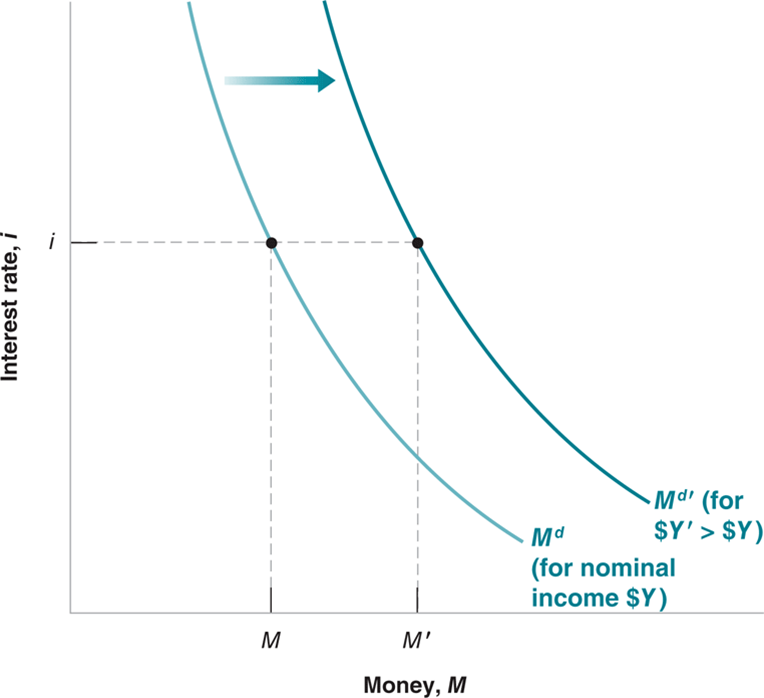
\includegraphics{graphs/L3F1.png}
    }
  }
\end{column}%
\end{columns}
\pause
%\begin{center}
\textbf{Summary:}
\begin{itemize}
\item[1] $\uparrow Y \Rightarrow \uparrow M^d $
\item[2] $\uparrow i \Rightarrow \downarrow M^d$
\end{itemize}
%\end{center}
\end{frame}

\section{Determining the Interest Rate}
%%%%%%%%%%%%%%%%%%%%%%%
\begin{frame}{Determining the Interest Rate}
\begin{columns}[T] % align columns
\begin{column}{.52\textwidth}
  \begin{wideitemize}
    \item At this point, let's just keep it simple. We assume that RBI supplies a fixed amount of money.
           \[ M^s = M \]
    \item $M^s = M^d$ is the condition for financial market equilibrium.
          \[ M = YL(i) \]
    \item This relationship is known as the $LM$ relation.
  \end{wideitemize}
\end{column}%
\pause
\hfill%
\begin{column}{.44\textwidth}
  \makebox[\linewidth][c]{
    \resizebox{\linewidth}{!}{
      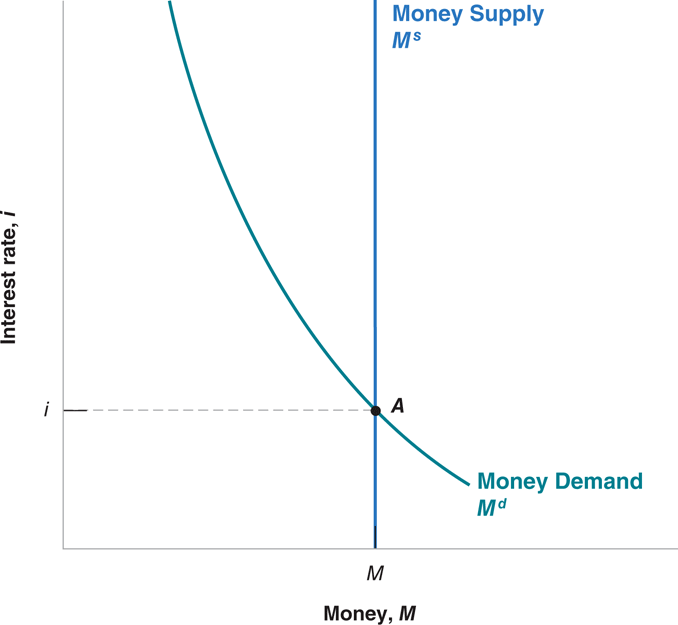
\includegraphics{graphs/L3F2.png}
    }
  }
\end{column}%
\end{columns}
\end{frame}

%%%%%%%%%%%%%%%%%
\begin{frame}{Shifts in Equilibrium}
\begin{columns}[T] % align columns
\begin{column}{.52\textwidth}
  \begin{wideitemize}
    \item $\uparrow Y$ \pause $\Rightarrow$ $\uparrow i$. \\
      \textit{An increase in nominal income leads to an increase in interest rate}
    \item What are the reasons? \pause
    \item At the initial interest rate, $M^d > M^s$. 
    \item An increase in interest rate is required to pull down the demand. 
  \end{wideitemize}
\end{column}%
\pause
\hfill%
\begin{column}{.44\textwidth}
  \makebox[\linewidth][c]{
    \resizebox{\linewidth}{!}{
      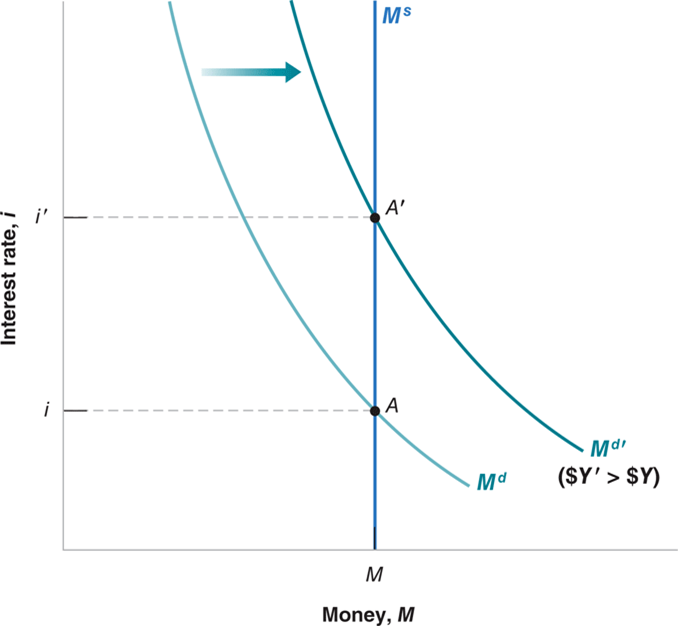
\includegraphics{graphs/L3F3.png}
    }
  }
\end{column}%
\end{columns}
\end{frame}

%%%%%%%%%%%%%%%%%%%%%%%%%%%%%%%%%
\begin{frame}{Shifts in Equilibrium}
\begin{columns}[T] % align columns
\begin{column}{.52\textwidth}
  \begin{wideitemize}
    \item $\uparrow M^s$ \pause $\Rightarrow$ $\downarrow i$. \\
      \textit{An increase in money supply leads to a fall in interest rate}
    \item What are the reasons? \pause
    \item At the initial interest rate, $M^s > M^d$. 
    \item A fall in interest rate is required to stimulate the demand. 
  \end{wideitemize}
\end{column}%
\pause
\hfill%
\begin{column}{.44\textwidth}
  \makebox[\linewidth][c]{
    \resizebox{\linewidth}{!}{
      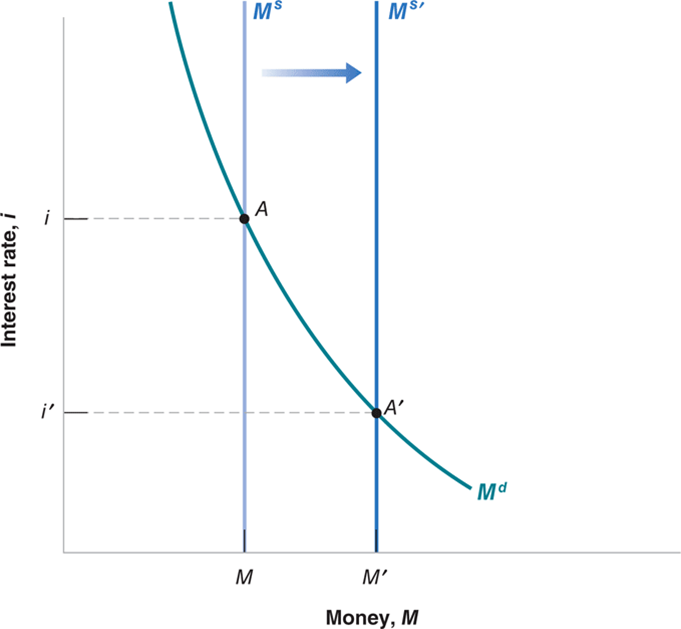
\includegraphics{graphs/L3F4.png}
    }
  }
\end{column}%
\end{columns}
\end{frame}

%%%%%%%%%%%%%%%%%%%%%
\begin{frame}{Monetary Policy and Open Market Operations}
How does the RBI change the money supply?
\\ \pause
\vspace{5mm}
\textbf{Open Market Operations (OMO):} Central banks buy and sell bonds in the bond market.
\vspace{3mm}

\begin{wideitemize}
\item \textcolor{red!90}{Expansionary OMO}: Central banks \textbf{buy} bonds.
\item \textcolor{red!90}{Contractionary OMO}: Central banks \textbf{sell} bonds.
\end{wideitemize}
\end{frame}

%%%%%%%%%%%%%%%%%%%%%
\begin{frame}{Bond Prices and Bond Yields}
\begin{wideitemize}
\item Assume that bonds are just one-year bonds which promise \rupee 100 a year from now.
\item Such bonds are known as \textcolor{red}{Treasury bills} or \textbf{T-bills}.
\item If the price of the bond $B$ is $P_B$, the the rate of return from holding the bond will be $(100 - P_B)/P_B$.
\item So, the interest rate on the bond will be \pause
    \[ i = \frac{100 - P_B}{P_B} \]
\item What will be the price of the bond? \pause
    \[ P_B = \frac{100}{1 + i} \]
\end{wideitemize}
\pause
\textbf{Question:} Think about central bank's purchase/selling of bonds in this framework.
\end{frame}

\section{Determining the Interest Rate Returns}
%%%%%%%%%%%%%%%%%%%%%
\begin{frame}{What Banks Do}
\begin{columns}[T] % align columns
\begin{column}{.52\textwidth}
  \begin{wideitemize}
    \item Banks receive funds from people and firms who can write a check to withdraw these funds.
    \item Therefore, these funds or \textit{checkable deposits} are a bank's \textcolor{red!90}{liabilities}.
    \pause
    \item Banks withhold some funds. They can park these funds either in cash or with the RBI.
    \item These reserves act as \textcolor{red!90}{assets}.
    \pause
    \item Loans disbursed also enter a bank's balance sheet's assets column.
  \end{wideitemize}
\end{column}%
\pause
\hfill%
\begin{column}{.44\textwidth}
  \makebox[\linewidth][c]{
    \resizebox{\linewidth}{!}{
      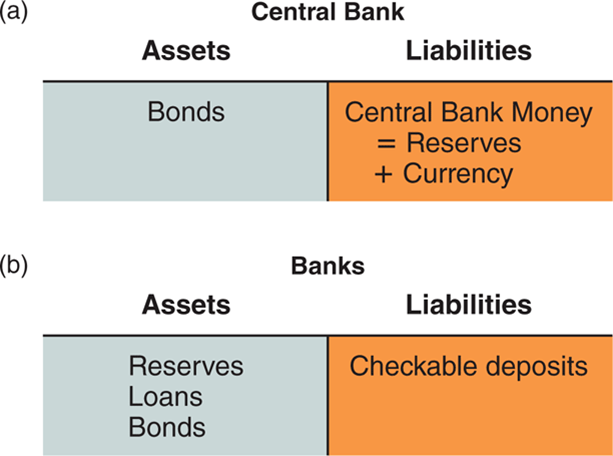
\includegraphics{graphs/L3F5.png}
    }
  }
\end{column}%
\end{columns}
\end{frame}

%%%%%%%%%%%%%%%%%%%%%%%%%%%%%%%%%%%
\begin{frame}{The Supply and the Demand for Central Bank Money}
We would want to understand now what determines..
\begin{wideitemize}
\item the demand for \textcolor{red}{checkable deposits} and the demand for \textcolor{red}{currency}?
\item the demand for reserves by banks?
\item the demand for central bank money?
\end{wideitemize}
\end{frame}

\begin{frame}
\makebox[\linewidth][c]{
    \resizebox{0.8\linewidth}{!}{
      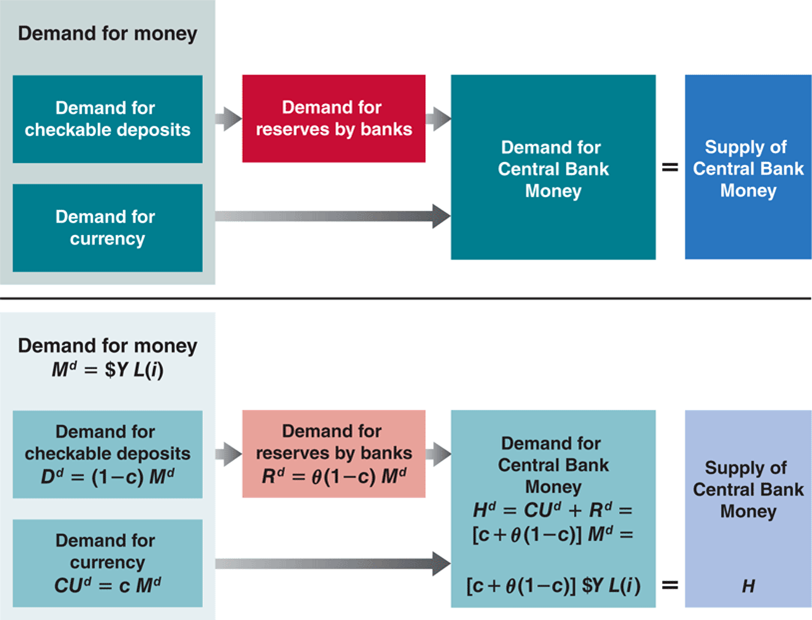
\includegraphics{graphs/L3F6.png}
    }}
\end{frame}

%%%%%%%%%%%%%%%%%%%%
\begin{frame}{The Demand for Money}
\begin{wideitemize}
\item Assumption: people hold their money in currency and deposits in fixed proportions.
\pause
\item The demand for currency: $CU^d = cM^d$.
\pause
\item The demand for deposits: $D = (1 - c)M^d$.
\end{wideitemize}
\end{frame}

%%%%%%%%%%%%%%%%%%%%
\begin{frame}{The Demand for Reserves}
\begin{wideitemize}
\item $\uparrow D^d$ $\Rightarrow$ $\uparrow$ amount of reserves ($R$) that banks must hold. (\textbf{Why?})
\item Let that fraction be $\theta$. So, the relationship between $R$ and $D$ is
     \[ R = \theta D \]
     \pause
     \[ R = \theta (1 - c)M^d \]
\end{wideitemize}
\end{frame}

%%%%%%%%%%%%%%%%%%%%
\begin{frame}{The Demand for Central Bank Money}
\begin{wideitemize}
\item Sum up currency and the deposit held by people, and you get the demand for central bank money ($H^d$). \pause
    \[ H^d = CU^d + R^d \]
\item Replace $CU^d$ and $R^d$ by the equations for demand for money. \pause
    \[ H^d = cM^d + \theta (1 - c)M^d \] \pause
    \[ H^d = [c + \theta (1 - c)]M^d \] \pause
    \[ H^d = [c + \theta (1 - c)]YL(i) \] 
\end{wideitemize}
\end{frame}

%%%%%%%%%%%%%%%%%%%%%%%%%%%%%%%%%%%%%%%
\begin{frame}{The Determination of the Interest Rate}
\begin{columns}[T] % align columns
\begin{column}{.52\textwidth}
  \begin{wideitemize}
    \item The equilibrium condition: 
         \[ H = H^d \]
    \pause
    \item \[ H = [c + \theta (1 - c)YL(i) \]
    \pause
    \item Think of extremes: $c = 1$ and $c = 0$.
  \end{wideitemize}
\end{column}%
\pause
\hfill%
\begin{column}{.44\textwidth}
  \makebox[\linewidth][c]{
    \resizebox{\linewidth}{!}{
      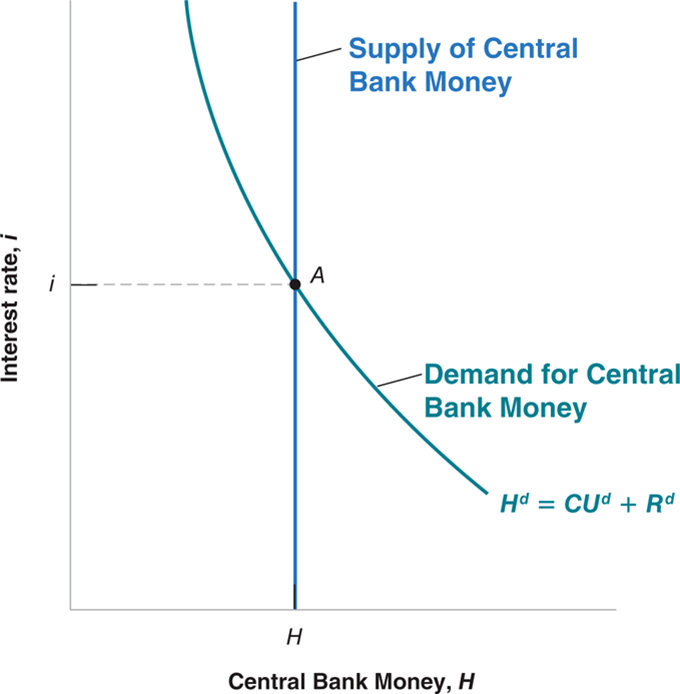
\includegraphics{graphs/L3F7.png}
    }
  }
\end{column}%
\end{columns}
\end{frame}


%%%%%%%%%%%%%%%%%%%%%%%%%%%%%%%%%%%%%%%
\begin{frame}
\frametitle{Mechanics of Central Banking}
Suppose there are no banks and there are just coins.
To be concrete, let's suppose that the total quantity of currency is Rs.100. The supply of
money is, therefore, Rs.100. \\
\vspace{3mm}
Let us suppose in this case that Nubia has Rs.100 in cash and she puts it in a bank account in Abacus Bank. \\
\vspace{3mm}
\begin{tabular}{cc}
\hline
Abacus Bank's assets &	Abacus Bank's liabilities \\
\hline
Base money	Rs.100	& Payable on demand to Nubia	Rs.100 \\
\hline
\end{tabular}
\\
\vspace{3mm}
After the bank opens and people deposit their currency, the money supply
is the Rs.100 of demand deposits.
\end{frame}


%%%%%%%%%%%%%%%%%%%%%%%%%%%%%%%%%%%%%%%
\begin{frame}
\frametitle{Mechanics of Central Banking}
Eventually, the bankers at Abacus Bank may start to reconsider their policy
of 100-percent-reserve banking. Leaving all that money idle in their vaults seems
unnecessary. Why not lend some of it out and earn a profit by charging interest
on the loans? \\
\vspace{3mm}
The fraction of total deposits that a bank holds as reserves is called the reserve
ratio. This ratio is determined by a combination of government regulation and
bank policy.\\
\vspace{3mm}
Let this ratio be 10 percent. 
\pause
\\
\vspace{3mm}
\begin{tabular}{cc}
\hline
%\multicolumn{2}{Abacus Bank} \\
Abacus Bank's assets &	Abacus Bank's liabilities \\
\hline
Loan Rs.90	& Deposits	Rs.100 \\
Reserve Rs.10 & \\
\hline
\end{tabular}
\end{frame}

%%%%%%%%%%%%%%%%%%%%%%%%%%%%%%%%%%%%%%%
\begin{frame}
\frametitle{Money Multiplier}
The creation of money does not stop with Abacus Bank. 
Suppose Nubia from Abacus uses the Rs.90 to buy groceries from Godot who then deposits the currency in Bonus Bank. \pause
\\
\vspace{3mm}
\begin{tabular}{cc}
\hline
%\multicolumn{2}{Abacus Bank} \\
Bonus Bank's assets &	Bonus Bank's liabilities \\
\hline
Loan Rs.81	& Deposits	Rs.90 \\
Reserve Rs.9 & \\
\hline
\end{tabular}
\end{frame}

%%%%%%%%%%%%%%%%%%%%%%%%%%%%%%%%%%%%%%%
\begin{frame}
\frametitle{Money Multiplier}
If Bonus also has a reserve ratio of 10 percent, it keeps assets of Rs.9 in reserve and makes Rs.81 in loans.
In this way, Bonus Bank creates an additional Rs.81 of money. If this Rs.81
is eventually deposited in Jackpot Bank, which also has a reserve ratio of
10 percent, this bank keeps Rs.8.10 in reserve and makes Rs.72.90 in loans. Here is the
T-account for Jackpot Bank: \pause
\\
\vspace{3mm}
\begin{tabular}{cc}
\hline
%\multicolumn{2}{Abacus Bank} \\
Jackpot Bank's assets & Jackpot Bank's liabilities \\
\hline
Loan Rs.72.9	& Deposits	Rs.81 \\
Reserve Rs.8.1 & \\
\hline
\end{tabular}
\end{frame}

\begin{frame}
The amount of money the banking system generates with
each rupee of reserves is called the money multiplier. In this imaginary economy,
where the Rs.100 of reserves generates Rs.1,000 of money, the money multiplier is 10. \\
\vspace{3mm}
What determines the size of the money multiplier? 
\\
\vspace{3mm}
\pause
It turns out that the answer
is simple: The money multiplier is the reciprocal of the reserve ratio. If R is the reserve
ratio for all banks in the economy, then each dollar of reserves generates 1/R dollars
of money. In our example, R = 1/10, so the money multiplier is 10.
\end{frame}

\end{document}